% Options for packages loaded elsewhere
\PassOptionsToPackage{unicode}{hyperref}
\PassOptionsToPackage{hyphens}{url}
\PassOptionsToPackage{dvipsnames,svgnames*,x11names*}{xcolor}
%
\documentclass[
  12pt,
]{book}
\usepackage{lmodern}
\usepackage{amssymb,amsmath}
\usepackage{ifxetex,ifluatex}
\ifnum 0\ifxetex 1\fi\ifluatex 1\fi=0 % if pdftex
  \usepackage[T1]{fontenc}
  \usepackage[utf8]{inputenc}
  \usepackage{textcomp} % provide euro and other symbols
\else % if luatex or xetex
  \usepackage{unicode-math}
  \defaultfontfeatures{Scale=MatchLowercase}
  \defaultfontfeatures[\rmfamily]{Ligatures=TeX,Scale=1}
  \setmonofont[]{Source Code Pro}
\fi
% Use upquote if available, for straight quotes in verbatim environments
\IfFileExists{upquote.sty}{\usepackage{upquote}}{}
\IfFileExists{microtype.sty}{% use microtype if available
  \usepackage[]{microtype}
  \UseMicrotypeSet[protrusion]{basicmath} % disable protrusion for tt fonts
}{}
\makeatletter
\@ifundefined{KOMAClassName}{% if non-KOMA class
  \IfFileExists{parskip.sty}{%
    \usepackage{parskip}
  }{% else
    \setlength{\parindent}{0pt}
    \setlength{\parskip}{6pt plus 2pt minus 1pt}}
}{% if KOMA class
  \KOMAoptions{parskip=half}}
\makeatother
\usepackage{xcolor}
\IfFileExists{xurl.sty}{\usepackage{xurl}}{} % add URL line breaks if available
\IfFileExists{bookmark.sty}{\usepackage{bookmark}}{\usepackage{hyperref}}
\hypersetup{
  pdftitle={Notas Curso de Estadística (Parte I)},
  pdfauthor={Maikol Solís},
  colorlinks=true,
  linkcolor=Maroon,
  filecolor=Maroon,
  citecolor=Blue,
  urlcolor=Blue,
  pdfcreator={LaTeX via pandoc}}
\urlstyle{same} % disable monospaced font for URLs
\usepackage{longtable,booktabs}
% Correct order of tables after \paragraph or \subparagraph
\usepackage{etoolbox}
\makeatletter
\patchcmd\longtable{\par}{\if@noskipsec\mbox{}\fi\par}{}{}
\makeatother
% Allow footnotes in longtable head/foot
\IfFileExists{footnotehyper.sty}{\usepackage{footnotehyper}}{\usepackage{footnote}}
\makesavenoteenv{longtable}
\usepackage{graphicx}
\makeatletter
\def\maxwidth{\ifdim\Gin@nat@width>\linewidth\linewidth\else\Gin@nat@width\fi}
\def\maxheight{\ifdim\Gin@nat@height>\textheight\textheight\else\Gin@nat@height\fi}
\makeatother
% Scale images if necessary, so that they will not overflow the page
% margins by default, and it is still possible to overwrite the defaults
% using explicit options in \includegraphics[width, height, ...]{}
\setkeys{Gin}{width=\maxwidth,height=\maxheight,keepaspectratio}
% Set default figure placement to htbp
\makeatletter
\def\fps@figure{htbp}
\makeatother
\setlength{\emergencystretch}{3em} % prevent overfull lines
\providecommand{\tightlist}{%
  \setlength{\itemsep}{0pt}\setlength{\parskip}{0pt}}
\setcounter{secnumdepth}{5}
%\usepackage{inputenc}
% \usepackage{newpxtext,newpxmath}
\setcounter{tocdepth}{3}
\setcounter{secnumdepth}{3}
\usepackage[spanish]{babel}
\usepackage{booktabs}
\usepackage{csquotes}
\usepackage{amsmath, amsthm, amssymb,amsbsy}
\usepackage{mathtools}
\usepackage{graphics, graphicx}

% \usepackage{setspace}
% \doublespacing
%\addbibresource{bibliografia.bib}


% \usepackage{tcolorbox}
% \tcbuselibrary{theorems}
% \tcbuselibrary{breakable}
% 
% \newtcbtheorem[number within=section]{nota}{Nota}%
% {breakable, colback=yellow!5, colframe=yellow!40!gray,
% 	fonttitle=\bfseries}{nota}
% 
% \newtcbtheorem[number within=section,use counter
% from=nota]{cuidado}{Cuidado}%
% {breakable, colback=red!5, colframe=red!50!gray,
% 	fonttitle=\bfseries}{cuidado}
% 
% \newtcbtheorem[number within=section,use counter
% from=nota]{tarea}{Tarea}%
% {breakable, colback=blue!5, colframe=blue!35!black,
% 	fonttitle=\bfseries}{tarea}
% 
% \newtcbtheorem[number within=section,use counter
% from=nota]{solucion}{Solución}%
% {breakable, colback=gray!5, colframe=gray!35!black,
% 	fonttitle=\bfseries}{sol}
% 
% \newtcbtheorem[number within=section,use counter
% from=nota]{pregunta}{Pregunta}%
% {breakable,  colback=green!5, colframe=green!35!black,
% 	fonttitle=\bfseries}{preg}
% 
% \newtcbtheorem[number within=section,use counter
% from=nota]{ejemplo}{Ejemplo}%
% {breakable, colback=magenta!10, colframe=magenta!50!black,
% 	fonttitle=\bfseries}{ej}
% 
% \newtcbtheorem[number within=section,use counter
% from=nota]{laboratorio}{Laboratorio}%
% {breakable, colback=purple!10, colframe=purple!50!black,
% 	fonttitle=\bfseries}{lab}
%%end novalidate

%
%\usepackage{amsmath}
%\usepackage{amsthm}
%\usepackage{amssymb}
%%%% DEFINICIÓN DE ESTILOS DE TEOREMAS %%%
%\theoremstyle{definition}
%\newtheorem{definicion}{Definición}
%
%\theoremstyle{plain}
%\newtheorem{teorema}{Teorema}
%\newtheorem{lema}{Lema}
%%%%%%%%%%%%%%%%%%%%%%%%%%%%%%%%%%%%%%%%%%
\usepackage[style=authoryear,url=false,doi=false,eprint=false,isbn=false]{biblatex}
\addbibresource{bibliografia.bib}

\title{Notas Curso de Estadística (Parte I)}
\author{Maikol Solís}
\date{Actualizado el 11 August, 2020}

\begin{document}
\maketitle

{
\hypersetup{linkcolor=}
\setcounter{tocdepth}{4}
\tableofcontents
}
\hypertarget{introducciuxf3n}{%
\chapter{Introducción}\label{introducciuxf3n}}

\hypertarget{inferencia-estaduxedstica}{%
\chapter{Inferencia estadística}\label{inferencia-estaduxedstica}}

\textbf{Definición:} Hacer afirmaciones probabilísticas respecto a (acerca de)
cantidades desconocidas.

\hypertarget{ejemplo}{%
\section{Ejemplo}\label{ejemplo}}

*\textbf{Pregunta}: ¿Será posible modelar cuánto dura un componente electrónico en
fallar?

\textbf{Solución}: Podemos responder esta pregunta dividiéndola en dos partes:

\begin{enumerate}
\def\labelenumi{\arabic{enumi}.}
\tightlist
\item
  \textbf{Modelo probabilístico:} Asuma que los tiempos de vida del componente son
  exponenciales (en años).
\item
  \textbf{Parámetro:} Sea \(\theta > 0\) la tasa de fallo (unidades: 1/Tiempo(años)).
\end{enumerate}

Es decir, tenemos un modelo (exponencial) y estamos decretando que su información estará concentrada en el parámetro \(\theta\).

\textbf{Nota}: El parámetro \(\theta\) contiene la información del modelo,
pero ¿Cómo obtenemos esa información

\textbf{Muestra}: Secuencia (sucesión) de variables aleatorias independientes \(X_1,X_2,\dots, X_n,\dots\). Tomemos una muestra \(X_1,X_2,\dots, X_n,\dots \stackrel{i.i.d}{\sim} \text{Exp}(\theta)\).

\textbf{Objetivos}

\begin{itemize}
\item
  Estimar \(X_m, X_{m+1}, \dots\) si se observa \(X_1, X_{m-1}, \dots\) (Predicción).
\item
  Estimar \(\theta\) usando información.
\end{itemize}

\textbf{Datos}: Realizaciones de variables aleatorias \(X_1,\dots,X_m\) pertenecientes a la muestra.

\textbf{Estimación de \(\theta\)}

Dado que \(\mathbb{E}(X) = \dfrac{1}{\theta}\) con \(X \sim \text{Exp}(\theta)\), por la ley de grandes números se tiene que

\begin{equation*}
\underbrace{\dfrac{1}{n} \sum_{i=1}{X_i}}_{\bar{X}_n} \xrightarrow[n\to \infty]{\mathbb{P}}\mathbb{E}(X) = \dfrac{1}{\theta}
\end{equation*}

por propiedad de convergencia en probabilidad.

Un posible candidato para estimar \(\theta\) es \(\dfrac{1}{\bar X_n}\), bajo el supuesto por Ley de Grandes Números que \(\theta\) es una constante (frecuentista).

\textbf{Realidad}: \(\theta\) no necesariamente es determinístico (factores externos, por la naturaleza del fenómeno).

Asumimos un modelo probabilístico para \(\theta\) (tasa siempre positiva):

\begin{equation*}
\theta \sim \Gamma(\alpha_0,\beta_0)
\end{equation*}
Luego, según estudios previos la tasa esperada es 0.5/año
\begin{equation*}
\mathbb{E}(\theta) = \dfrac{1}{2} = \dfrac{\alpha_0}{\beta_0}.
\end{equation*}

Un primer indicio de que se podría establecer que \(\alpha_0 = 1\) y de \(\beta_0 = 2\).

\hypertarget{modelo-estaduxedstico}{%
\section{Modelo estadístico}\label{modelo-estaduxedstico}}

Vamos a definir como típicamente se define un modelo estadístico.

\begin{enumerate}
\def\labelenumi{\arabic{enumi}.}
\item
  Variables aleatorias observables / hipotéticamente observables:

  \begin{equation*}
    \underbrace{X_t}_{\text{Observable}} = \underbrace{Y_t}_{\text{Hip. observable}} + \underbrace{\epsilon}_{\text{Ruido}}
    \end{equation*}

  En otras palabras \(Y_t\) sería la el dato \emph{``verdadero''} que pasó
  exactamente en el fenómeno analizado. Esta observación es afectada por
  muchos factores no observables (por ejemplo: errores de medición, cambio
  de las condiciones de la economía, etc.). La variable \(\epsilon\) captura
  toda esa aleatoriedad que no es parte del fénomeno.

  Claramente ni \(Y_t\) ni \(\epsilon\) se pueden medir y la mejor
  representación del nuestro es fenómeno es a partir de \(X_t\).
\item
  Distribución conjunta de una muestra de variables observables.

  Es decir cuál es el supuesto general que estoy usando para describir mis
  observaciones.
\item
  Parámetros que son hipotéticamente observables (desconocidos).

  ¿Cuál sería la mejor calibración de los componentes del modelo anterior de
  modo que mi modelo se ajuste a los datos?
\item
  (Opcional) Distribución conjunta de los parámetros.

  En el caso de Bayes, los parámetro dejan de ser simple valores puntuales y se
  convierten en distribuciones completas.
\end{enumerate}

\begin{itemize}
\tightlist
\item
  \textbf{Inferencia estadística}: procedimiento que genera afirmaciones probabilísticas de un modelo estadístico.
\end{itemize}

\textbf{Ejemplo de inferencias}:

\begin{enumerate}
\def\labelenumi{\arabic{enumi}.}
\item
  Estimar \(\theta\) a través de \(\dfrac{1}{\bar X_n}\).
\item
  ¿Qué tan probable es que el promedio de las siguientes observaciones es al menos 2?
  \begin{equation*}
  \dfrac{1}{10}\sum_{i= m+1}^{m+10} X_i > 2
  \end{equation*}
\item
  ¿Qué tan cierto es que \(\theta\leq0.4\) después de observar la muestra?
\end{enumerate}

\begin{itemize}
\item
  \textbf{Parámetro}: característica (s) que determinan la distribución conjunta de las variables aleatorias de interés.
\item
  \textbf{Espacio paramétrico} \(\Omega\) (espacio de parámetros, puede ser de probabilidad)
\end{itemize}

\textbf{Ejemplos}:

\begin{itemize}
\tightlist
\item
  \(\theta\) \textgreater{} 0 (ejemplo anterior); \(\Omega = (0,+\infty)\).
\item
  \(X_1,\dots,X_n \sim N(\mu, \sigma^2)\), \((\mu,\sigma^2)\) parámetros; \(\Omega\) = \(\mathbb{R}\times[0,+\infty)\).
\end{itemize}

\textbf{Ejemplo:} Clientes de un banco

¿Qué tan probable es que un cliente no pague su crédito hoy?

\begin{itemize}
\item
  \textbf{Datos}: \(X_i = \begin{cases}1& \text{el cliente } \#i \text{ no pagó}\\0 & \text{el cliente } \#i \text{ pagó}\end{cases}\).
\item
  \textbf{Muestra}: \(X_1,\dots,X_{10000}\) (realización al día de hoy).
\item
  \textbf{Modelos}: \(X_1,\dots, X_{10000} \stackrel{i.i.d}{\sim} \text{Ber}(p)\) con \(p\in[0,1]\).
\item
  \textbf{Parámetro}: \(p\), \(\Omega = [0,1]\).
\item
  \textbf{Inferencias:}

  \begin{itemize}
  \tightlist
  \item
    Estimar \(p\) (probabilidad de impago).
  \item
    Suponga que \(L(X_i)\) es el saldo en la cuenta del cliente \(\#i\).
  \end{itemize}
\end{itemize}

\begin{equation*}
\mathbb{P}\left(\sum_{i=1}^{10000}L(X_i)>u\right)=\text{Probabilidad de ruina}
\end{equation*}

\hypertarget{estaduxedstico}{%
\section{Estadístico}\label{estaduxedstico}}

\textbf{Definición}. Si \(X_1,\dots,X_n\) es una muestra observable. Sea \(r\) una función real de \(n\) variables:
\begin{equation*}
T = r(X_1,\dots,X_n)
\end{equation*}
es un estadístico.

\textbf{Nota}: \(T\) también es aleatorio.

\textbf{Ejemplos}:

\begin{itemize}
\item
  \(\hat p = \dfrac{1}{10000}\displaystyle\sum_{i=1}^{10000}X_i = \dfrac{\#\text{ no pagan}}{\text{Total}} = r(X_1,\dots,X_{10000})\)
\item
  \(L_m = \max L(X_i)\) (saldo del cliente más riesgoso).
\item
  \(R_m = \max L(X_i) - \min L(X_i), 1\leq i\leq 10000\)
\end{itemize}

\hypertarget{distribuciuxf3n-previa-distribuciuxf3n-a-priori}{%
\chapter{Distribución previa (distribución a priori)}\label{distribuciuxf3n-previa-distribuciuxf3n-a-priori}}

Suponga que tenemos un modelo estadístico con parámetro \(\theta\). Su \(\theta\) es aleatorio entonces su densidad (antes de observar cualquier muestra) se llama \textbf{densidad previa}: \(\pi\).

\textbf{Ejemplo}: \(X_1,\dots, X_n \sim \text{Exp}(\theta)\) y \(\theta\) es aleatorio tal que \(\theta \sim \Gamma(\stackrel{\alpha}{1},\stackrel{\beta}{2})\) entonces

\[ \pi(\theta) = \dfrac{1}{\Gamma(\alpha)}\beta^\alpha\theta^{\alpha-1}e^{\beta\theta} = 2e^{-2\theta}, \quad \theta > 0\]

\textbf{Ejemplo}: Sea \(\theta\) la probabilidad de obtener cara al tirar una moneda.

\begin{itemize}
\item
  Moneda justa: \(\theta = \dfrac{1}{2}\) con probabilidad previa \(0.8\) (\(\pi(\frac{1}{2}) = 0.8\)).
\item
  Moneda de dos caras: \(\theta = 1\) con probabilidad previa \(0.2\) (\(\pi(1) = 0.2\)).
\end{itemize}

\textbf{Notas}:

\begin{itemize}
\item
  \(\pi\) está definida en \(\Omega\) (espacio paramétrico).
\item
  \(\pi\) es definida antes de obtener la muestra.
\end{itemize}

\textbf{Ejemplo} (Componentes eléctricos)

Criterio experto: \(\mathbb{E}[\theta] = 0.0002^K\), \(\sqrt{\text{Var}(\theta)} = 0.0001^K\).

Bajo la misma densidad \(\pi\):
\[ \mathbb{E}[\theta] = \dfrac{\alpha}{\beta}, \text{Var}(\theta) = \dfrac{\alpha}{\beta^2}\]

\[\implies \begin{cases}\dfrac{\alpha}{\beta} = 2\times 10^{-4}\\\sqrt{\dfrac{\alpha}{\beta^2}} = 1 \times 10^{-4}\end{cases} \implies \beta = 20000, \alpha = 4\]

\textbf{Notación}:

\begin{itemize}
\item
  \(X = (X_1,\dots, X_n)\): vector que contiene la muestra aleatoria.
\item
  Densidad conjunta de \(X\): \(f_\theta(x)\).
\item
  Densidad de \(X\) condicional en \(\theta\): \(f_n(x|\theta)\).
\end{itemize}

\textbf{Supuesto}: \(x\) viene de una muestra aleatoria si y solo si \(X\) es condicionalmente independiente dado \(\theta\).

\textbf{Consecuencia}: \[f_n(X|\theta) = f(X_1|\theta)\cdot f(X_2|\theta)\cdots f(X_n|\theta)\]

\textbf{Ejemplo}

Si \(X = (X_1,\dots, X_n)\) es una muestra tal que \(X_i\sim \text{Exp}(\theta)\),
\[ f_n(X|\theta) = \begin{cases}\prod_{i=1}^n \theta e^{-\theta X_i} & \text{si } X_i>0\\
0 & \text{si no}
\end{cases} = \begin{cases}\theta^n e^{-\theta\sum_{i=1}^n X_i} & X_i > 0 \forall i\\ 0 & \text{si no}\end{cases}\]

\hypertarget{densidad-posterior}{%
\section{Densidad posterior}\label{densidad-posterior}}

\textbf{Definición}. Considere un modelo estadístico con parámetro \(\theta\) y muestra aleatoria \(X_1,\dots, X_n\). La densidad condicional de \(\theta\) dado \(X_1,\dots,X_n\) se llama \emph{densidad posterior}: \(\pi(\theta|X)\)

\textbf{Teorema}. Bajo las condiciones anteriores:
\[\pi(\theta|X) = \dfrac{f(X_1|\theta)\cdots f(X_n|\theta)\pi(\theta)}{g_n(X)}\]
para \(\theta \in \Omega\), donde \(g_n\) es una constante de normalización.

\emph{Prueba}:
\begin{align*}
\pi(\theta|X) & = \dfrac{\pi(\theta,X)}{\text{marginal de X}} = \dfrac{\pi(\theta,X)}{\int \pi(\theta,X)\;d\theta}= \dfrac{P(X|\theta)\cdot \pi(\theta)}{\int \pi(\theta,X)\;d\theta}\\
& \dfrac{f_n(X|\theta)\cdot \pi(\theta)}{g_n(X)} = \dfrac{f(X_1|\theta)\cdots f(X_n|\theta)\pi(\theta)}{g_n(X)}
\end{align*}

Del ejemplo anterior,

\[f_n(X|\theta) = \theta^n e^{-\theta y}, y = \sum{X_i} \text{ (estadístico})\]
Numerador:

\[f_n(X|\theta)\pi(\theta) = \underbrace{\theta^n e^{-\theta y}}_{f_n(X|\theta)} \cdot \underbrace{\dfrac{200000^4}{3!}\theta^3e^{-20000\cdot\theta}}_{\pi(\theta)} = \dfrac{20000^4}{3!}\theta^{n+3}e^{(20000+y)\theta}\]

Denominador:

\[g_n(x) = \int_{0}^{+\infty}\theta^{n+3}e^{-(20000+y)\theta}\;d\theta = \dfrac{\Gamma(n+4)}{(20000+y)^{n+4}}\]

Entonces la posterior corresponde a
\[\pi(\theta|X) = \dfrac{\theta^{n+3}e^{-(20000+y)\theta}}{\Gamma(n+4)} (20000+y)^{n+4}\]
que es una \(\Gamma(n+4,20000+y)\).

Con 5 observaciones (horas): 2911, 3403, 3237, 3509, 3118.
\[y = \sum_{i=1}^{5}X_i = 16478, \quad n= 5\]
por lo que \(\theta|X \sim \Gamma(9,36178)\)

\begin{center}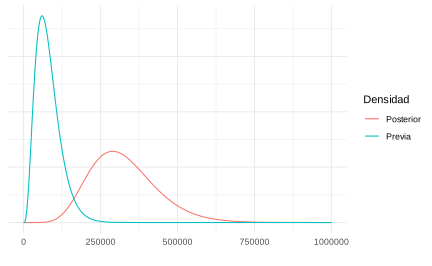
\includegraphics[width=0.7\linewidth]{Notas-Curso-Estadistica_files/figure-latex/unnamed-chunk-4-1} \end{center}

Es sensible al tamaño de la muestra (una muestra grande implica un efecto de la previa menor).

\textbf{Hiperparámetros}: parámetros de la previa o posterior.

\hypertarget{funciuxf3n-de-verosimilitud}{%
\section{Función de verosimilitud}\label{funciuxf3n-de-verosimilitud}}

Bajo el modelo estadístico anterior a \(f_n(X|\theta)\) se le llama \textbf{verosimilitud} o \textbf{función de verosimilitud}.

\textbf{Observación}. En el caso de una función de verosimilitud, el argumento es \(\theta\).

\textbf{Ejemplo}.

Sea \(\theta\) la proporción de aparatos defectuosos, con \(\theta \in [0,1]\)
\[ X_i = \begin{cases}1 & \text{falló} \\ 2 & \text{no falló}\end{cases}\]

\(\{X_i\}_{i=1}^n\) es una muestra aleatoria y \(X_i \sim Ber(\theta)\).

\begin{itemize}
\tightlist
\item
  \textbf{Verosimilitud}
\end{itemize}

\[ f_n(X|\theta) = \prod_{i=1}^n f(X_i|\theta) = \begin{cases}\theta^{\sum X_i}(1-\theta)^{n-\sum X_i} & X_i = 0,1\; \forall i\\ 0 & \text{si no}\end{cases}\]

\begin{itemize}
\item
  \textbf{Previa}:
  \[\pi(\theta) = 1_{\{0\leq\theta\leq 1\}}\]
\item
  \textbf{Posterior}:
\end{itemize}

Por el teorema de Bayes,
\[\pi(\theta|X) \propto \theta^y (1-\theta)^{n-y}\cdot 1 = \theta^{\overbrace{y+1}^{\alpha}-1}(1-\theta)^{\overbrace{n-y+1}^{\beta}-1} \implies \theta|X \sim \text{Beta}(y+1,n-y+1)\]

\begin{itemize}
\tightlist
\item
  \textbf{Predicción}.
\end{itemize}

\emph{Supuesto}: los datos son secuenciales. Calculamos la distribución posterior secuencialmente:
\begin{align*}
\pi(\theta|X_1) & \propto \pi(\theta) f(X_1|\theta)\\
\pi(\theta|X_1,X_2) &\propto \pi(\theta) f(X_1,X_2|\theta) = \pi(\theta) f(X_1|\theta) f(X_2|\theta) \text{ (por independencia condicional)}
\\ & = \pi(\theta|X_1)f(X_2|\theta)\\
\vdots &  \\
\pi(\theta|X_1,\dots,X_n) & \propto f(X_n|\theta)\pi(\theta|X_1,\dots, X_{n-1})
\end{align*}

Bajo independencia condicional no hay diferencia en la posterior si los datos son secuenciales.

Luego,

\begin{align*} 
g_n(X) & = \int_{\Omega} f(X_n|\theta) \pi(\theta|X_1,\dots, X_{n-1})\;d\theta\\
& = P(X_n|X_1,\dots,X_{n-1}) \text{ (Predicción para }X_n)
\end{align*}

Continuando con el ejemplo de los artefactos, \(P(X_6>3000|X_1,X_2,X_3,X_4,X_5)\). Se necesita calcular \(f(X_6|X)\). Dado que
\[ \pi(\theta|X) = 2.6\times 10^{36}\theta^8 e^{-36178\theta}\]

se tiene

\[ f(X_6|X) = 2.6\times 10^{36} \int_{0}^1 \underbrace{\theta e^{-\theta X_6}}_{\text{Densidad de } X_6}\theta^8 e^{-36178\theta}\;d\theta = \dfrac{9.55 \times 10^{41}}{(X_6+36178)^{10}}\]
Entonces,
\[ P(X_6>3000) = \int_{3000}^{\infty} \dfrac{9.55\times10^{41}}{(X_6+36178)^{10}}\; dX_6 = 0.4882\]

La vida media se calcula como \(\dfrac{1}{2} = P(X_6>u|X)\).

\hypertarget{familias-conjugadas}{%
\section{Familias conjugadas}\label{familias-conjugadas}}

\textbf{Definición}. Sea \(X_1,\dots, X_n\) i.i.d. condicional dado \(\theta\) con densidad \(f(X|\theta)\). Sea \(\psi\) la familia de posibles densidades previas sobre \(\Omega\). Si, sin importar los datos, la posterior pertenece a \(\psi\), entonces decimos que \(\psi\) es una familia conjugada de previas.

\textbf{Ejemplos}:

\begin{itemize}
\item
  La familia Beta es familia conjugada para muestras según una Bernoulli.
\item
  La familia Gama es familia conjugada para muestras exponenciales.
\item
  Para el caso Poisson, si \(X_1,\dots,X_n\sim Poi(\lambda)\),entonces la familia Gamma es familia conjugada.
\end{itemize}

La función de densidad de una Poisson es \(P(X_i = k) = e^{-\lambda}\dfrac{\lambda^k}{k!}\). La verosimilitud corresponde a
\[ f_n(X|\lambda) = \prod_{i=1}^{n}e^{-\lambda}\dfrac{\lambda^X_i}{X_i!} = \dfrac{e^{-n\lambda\lambda^y}}{\prod_{i=1}^n X_i}.\]
La previa de \(\lambda\) está definida por \(\pi(\lambda)\propto\lambda^{\alpha-1}e^{-\beta\lambda}\). Por lo tanto, la posterior es
\[ \pi(\lambda|X) \propto \lambda^{y+\alpha-1}e^{-(\beta+n)\lambda} \implies \lambda|X \sim \Gamma(y+\alpha,\beta+n)\]

\begin{itemize}
\tightlist
\item
  En el caso normal, si \(X_1,\dots,X_n\sim N(\theta,\sigma^2)\),entonces la familia normal es conjugada si \(\sigma^2\) es conocido.
\end{itemize}

Si \(\theta \sim N(\mu_0,V_0^2) \implies \theta|X \sim N(\mu_1, V_1^2)\) donde,
\[\mu_1 = \dfrac{\sigma^2\mu_0 + nV_0^2 \bar X_n}{\sigma^2 + nV_0^2}  = \dfrac{\sigma^2}{\sigma^2 + nV_0^2}\mu_0 + \dfrac{nV_0^2}{\sigma^2 + nV_0^2}\bar X_n\]

Combina de manera ponderada la previa y la de los datos.

\textbf{Ejemplo 7.3.6}

Considere una verosimilitud Poisson(\(\lambda\)) y una previa
\[ \pi(\lambda) = \begin{cases}2e^{-2\lambda} & \lambda> 0 \\ 0 & \lambda \geq 0\end{cases} \quad \lambda \sim \Gamma(1,2)\]

Supongamos que es una muestra aleatoria de tamaño \(n\). ¿Cuál es el número de observciones para reducir la varianza, a lo sumo, a 0.01?

Por teorema de Bayes, la posterior \(\lambda|x \sim \Gamma(y+1,n+2)\). Luego, la varianza de la Gamma es
\[\dfrac{\alpha}{\beta^2} = \dfrac{\sum x_i + 1}{(n+2)^2} \leq 0.01 \implies \dfrac{1}{(n+2)^2} \leq \dfrac{\sum x_i + 1}{(n+2)^2} \leq 0.01 \implies 100 \leq (n+2)^2 \implies n\geq 8\]
\textbf{Teorema}. Si \(X_1,\dots,X_n \sim N(\theta, \sigma^2)\) con \(\sigma^2\) conocido y la previa es \(\theta \sim N(\mu_0,V_0^2)\), entonces \(\theta|X\sim N(\mu_1,V_1^2)\) donde
\[ \mu_1 =  \dfrac{\sigma^2\mu_0 + nV_0^2 \bar X_n}{\sigma^2 + nV_0^2}, \quad V_1^2 = \dfrac{\sigma^2V_0^2}{\sigma^2 + nV_0^2}\]

\emph{Prueba}:

\begin{itemize}
\tightlist
\item
  \textbf{Verosimilitud}:
\end{itemize}

\[ f_n(X|\theta) \propto \exp\left[- \dfrac{1}{2\sigma^2} \sum_{i=1}^{n}(X_i\theta)^2\right]\]
Luego,
\begin{align*}
\sum_{i=1}^n (X_i-\theta)^2 & = \sum_{i=1}^n (X_i-\bar X + \bar X - \theta)^2 \\
& = n(\bar X + \theta)^2 + \sum_{i=1}^n (X_i-\bar X)^2 + \underbrace{2 \sum_{i=1}^n (X_i-\bar X)(\bar X - \theta)}_{= 0 \text{ pues } \sum Xi = n\bar X)}
\end{align*}
Entonces
\[ f_n(X|\theta) \propto \exp\left[-\dfrac{n}{2\sigma ^2}(\bar X - \theta )^2\right].\]

\begin{itemize}
\tightlist
\item
  \textbf{Previa}:
\end{itemize}

\[ \pi(\theta) \propto \exp\left[-\dfrac{1}{2V_0^2}(\theta - \mu_0)^2\right].\]

\begin{itemize}
\tightlist
\item
  \textbf{Posterior}:
\end{itemize}

\[ \pi(\theta|X) \propto \exp\left[-\dfrac{n}{2\sigma ^2}(\bar X - \theta )^2-\dfrac{1}{2V_0^2}(\theta - \mu_0)^2\right].\]

Con \(\mu_1\) y \(V_1^2\) definidos anteriormente, se puede comprobar la siguiente identidad:

\[-\dfrac{n}{\sigma ^2}(\bar X - \theta )^2-\dfrac{1}{V_0^2}(\theta - \mu_0)^2= \dfrac{1}{V_1^2}(\theta-\mu_1)^2 + \underbrace{\dfrac{n}{\sigma^2 + nV_0^2}(\bar X_n- \mu_0)^2}_{\text{Constante con respecto a }\theta}\]
Por lo tanto, \[\pi(\theta|X) \propto \exp\left[-\dfrac{n}{2V_1^2}(\theta -\mu_1)^2\right]\]

\emph{Media posterior}:

\[\mu_1 = \underbrace{\dfrac{\sigma^2}{\sigma^2 + nV_0^2}}_{W_1}\mu_0 + \underbrace{\dfrac{nV_0^2}{\sigma^2 + nV_0^2}}_{W_2}
\bar X_n \]

\textbf{Afirmaciones}:

\begin{enumerate}
\def\labelenumi{\arabic{enumi})}
\item
  Si \(V_0^2\) y \(\sigma^2\) son fijos, entonces \(W_1 \xrightarrow[n\to \infty]{}0\) (la importancia de la media empírica crece conforme aumenta \(n\)).
\item
  Si \(V_0^2\) y \(n\) son fijos, entonces \(W_2 \xrightarrow[\sigma^2\to \infty]{}0\) (la importancia de la media empírica decrece conforme la muestra es menos precisa).
\item
  Si \(\sigma^2\) y \(n\) son fijos, entonces \(W_2 \xrightarrow[V_0^2\to \infty]{}1\) (la importancia de la media empírica crece conforma la previa es menos precisa).
\end{enumerate}

\textbf{Ejemplo (determinación de n)}

Sean \(X_1,\dots, X_n \sim N(\theta,1)\) y \(\theta\sim N(\mu_0,4)\). Sabemos que \[V_1^2 = \dfrac{\sigma^2V_0^2}{\sigma^2 + nV_0^2}. \]
Buscamos que \(V_1\leq 0.01\), entonces
\[ \dfrac{4}{4n+1}\leq 0.01 \implies n\geq 99.75 \text{ (al menos 100 observaciones)}\]

\hypertarget{densidades-previas-impropias}{%
\section{Densidades previas impropias}\label{densidades-previas-impropias}}

\textbf{Definición}. Sea \(\pi\) una función positiva cuyo dominio está en \(\Omega\). Suponga que \(\int\pi(\theta)\;d\theta = \infty\). Entonces decimos que \(\pi\) es una \textbf{densidad impropia}.

\textbf{Ejemplo}: \(\theta \sim \text{Unif}(\mathbb{R})\), \(\lambda \sim \text{Unif}(0,\infty)\).

Una técnica para seleccionar distribuciones impropia es sustituir los hiperparámetros previos por 0.

\textbf{Ejemplo}:

Se presenta el número de soldados prusianos muertos por una patada de caballo (280 conteros, unidades de combate en 20 años).

\begin{longtable}[]{@{}ll@{}}
\toprule
Unidades & Ocurrencias\tabularnewline
\midrule
\endhead
144 & 0\tabularnewline
91 & 1\tabularnewline
32 & 2\tabularnewline
11 & 3\tabularnewline
2 & 4\tabularnewline
\bottomrule
\end{longtable}

\begin{itemize}
\item
  Muestra de Poisson: \(X_1 = 0, X_2 = 1, X_3 = 1,\dots, X_{280} = 0 \sim \text{Poi}(\lambda)\).
\item
  Previa: \(\lambda \sim \Gamma(\alpha, \beta)\).
\item
  Posterior: \(\lambda|X \sim \Gamma(y+\alpha, n+\beta) = \Gamma(196 + \alpha, 280 + \beta)\).
\end{itemize}

Sustituyendo,
\[\alpha=\beta = 0 \implies \pi(\lambda) \propto \lambda_{\alpha-1}e^{-\lambda\beta} = \dfrac{1}{\lambda}\]
donde \(\displaystyle\int_{0}^{\infty}\dfrac{1}{\lambda} d\lambda = \infty\).

Por teorema de Bayes, \[\theta|X \sim \Gamma(196,280)\]

\hypertarget{funciones-de-puxe9rdida}{%
\section{Funciones de pérdida}\label{funciones-de-puxe9rdida}}

\textbf{Definición}. Sean \(X_1,\dots, X_n\) datos observables cuyo modelo está indexado por \(\theta\in\Omega\). Un estimador de \(\theta\) es cualquier estadístico \(\delta(X_1,\dots, X_n)\).

\textbf{Notación}:

\begin{itemize}
\tightlist
\item
  Estimador \(\to \delta(X_1,\dots,X_n)\).
\item
  Estimación o estimado: \(\delta(X_1,\dots,X_n)(\omega) = \delta(\overbrace{x_1,\dots,x_n}^{datos})\)
\end{itemize}

\textbf{Definición}. Una \textbf{función de pérdida} es una función de dos variables:
\[ L(\theta,a), \quad \theta \in\Omega\]
con \(a\) un número real.

\textbf{Interpretación}: es lo que pierde un analista cuando el parámetro es \(\theta\) y el estimador es \(a\).

Asuma que \(\theta\) tiene una previa. La pérdida esperada es
\[ \mathbb{E}[L(\theta,a)] = \int_{\Omega}L(\theta, a) \pi(\theta)\;d\theta\]
la cual es una función de \(a\), que a su vez es función de \(X_1,\dots,X_n\). Asuma que \(a\) se selecciona el minimizar esta esperanza. A ese estimador \(a = \delta^*(X_1,\dots, X_n)\) se le llama \textbf{estimador bayesiano}, si ponderamos los parámetros con respecto a la posterior.

\[\mathbb{E}[L(\theta, \delta^*)|X] = \int_{\Omega}L(\theta, a) \pi(\theta)\;d\theta = \min_a \mathbb{E}[L(\theta|a)X]. \]

\hypertarget{funciuxf3n-de-puxe9rdida-cuadruxe1tica}{%
\subsection{Función de pérdida cuadrática}\label{funciuxf3n-de-puxe9rdida-cuadruxe1tica}}

\[ L(\theta, a) = (\theta-a)^2\]

En el caso en que \(\theta\) es real y \(\mathbb{E}[\theta|X]\) es finita, entonces
\[ \delta^*(X_1,\dots, X_n) = \mathbb{E}[\theta|X] \text{ cuando } L(\theta,a) = (\theta-a)^2. \]

\textbf{Ejemplo}: \(X_1,\dots, X_n \sim \text{Ber}(\theta)\), \(\theta \sim \text{Beta}(\alpha,\beta) \implies \theta|X \sim \text{Beta}(\alpha+y,\beta+n-y)\).

El estimador de \(\theta\) es
\[ \delta^*(X_1,\dots, X_n) = \dfrac{\alpha+y}{\alpha + \beta + n} = \overbrace{\dfrac{\alpha}{\alpha + \beta} }^{\text{Esperanza previa}}\cdot \dfrac{\alpha +\beta}{\alpha +\beta + n} + \overbrace{\dfrac{y}{n}}^{\bar X}\cdot \dfrac{n}{\alpha +\beta + n}.  \]

\hypertarget{funciuxf3n-de-puxe9rdida-absoluta}{%
\subsection{Función de pérdida absoluta}\label{funciuxf3n-de-puxe9rdida-absoluta}}

\[ L(\theta,a) = |\theta-a|\]

La pérdida esperada es
\[ f(a) = \mathbb{E}[L(\theta,a)|X] = \int_{-\infty}^{+\infty}|\theta-a|\pi(\theta|X)\;d\theta = \int_{a}^{+\infty}(\theta-a)\pi(\theta|X)\;d\theta + \int_{-\infty}^{a}(a-\theta)\pi(\theta|X)\;d\theta \]

Usando el teorema fundamental del cálculo,
\[F_{\pi}(a|X) = \int_{-\infty}^{\hat a}\pi(\theta|X)\;d\theta = \dfrac12 \Leftrightarrow \hat a= \operatorname*{argmin}_a f(a)\]

La \textbf{mediana} es el punto de \(X_{0.5}\) tal que \(F(X_{0.5}) = \dfrac{1}{2}\).

\textbf{Corolario}. Bajo la función de pérdida absoluta, el estimador bayesiano es la mediana posterior.

\textbf{Ejemplo}: Bernoulli.
\[ \dfrac{1}{\text{Beta}(\alpha+y, \beta+n-y)}\int_{-\infty}^{X_{0.5}}\theta^{\alpha+y-1} (1-\theta)^{\beta+n-y-1}\;d\theta = \dfrac12\]
Resuelva para \(X_{0.5}\).

\hypertarget{otras-funciones-de-puxe9rdida}{%
\subsection{Otras funciones de pérdida}\label{otras-funciones-de-puxe9rdida}}

\begin{itemize}
\item
  \(L(\theta,a) = |\theta-a|^k\), \(k\ne 1,2\), \(0<k<1\).
\item
  \(L(\theta,a) = \lambda(\theta)|\theta-a|^2\) (\(\lambda(\theta)\) penaliza la magnitud del parámetro).
\item
  \(L(\theta,a)=\begin{cases}3(\theta-a)^2 & \theta\leq a \text{ (sobreestima)}\\ (\theta-a)^2&\theta\geq a \text{ (subestima)} \end{cases}\)
\end{itemize}

\hypertarget{efecto-de-muestras-grandes}{%
\section{Efecto de muestras grandes}\label{efecto-de-muestras-grandes}}

\textbf{Ejemplo}: ítemes malos (proporción: \(\theta\)), \(\theta \in [0,1]\). Función de pérdida cuadrática. El tamaño de muestra son \(n=100\) ítemes, de los cuales \(y=10\) están malos.

\[ X_1,\dots,X_n\sim \text{Ber}(\theta)\]

\begin{itemize}
\tightlist
\item
  Primer previa. \(\alpha = \beta = 1\) (Beta). El estimador bayesiano corresponde a
\end{itemize}

\[ \mathbb{E}[\theta|X] = \dfrac{\alpha+y}{\alpha+\beta+n} = \dfrac{1+10}{2+100} = 0.108\]

\begin{itemize}
\tightlist
\item
  Segunda previa. \(\alpha =1, \beta=2 \implies \pi(\theta) = 2e^{-2\theta}, \theta >0\).
\end{itemize}

\[ \mathbb{E}[\theta|X] = \dfrac{1+10}{1+2+100} = \dfrac{11}{103}=0.107\]

La media es \(\bar X_n = \dfrac{10}{100} = 0.1\).

\hypertarget{consistencia}{%
\section{Consistencia}\label{consistencia}}

\textbf{Definición}. Un estimador de \(\theta\) \(\delta(X_1,\dots, X_n)\) es consistente si \[\delta(X_1,\dots, X_n)\xrightarrow[n\to \infty]{\mathbb{P}}\theta.\]

Bajo pérdida cuadrática, \(\mathbb{E}[\theta|X] = W_1\mathbb{E}[\theta] + X_2\bar X_n = \delta^*\). Sabemos, por ley de grandes números, que \(\bar X_n \xrightarrow[n\to \infty]{\mathbb{P}}\theta\). Además, \(W_1\xrightarrow[n\to \infty]{}0\) y \(W_2\xrightarrow[n\to \infty]{}1\).

En los ejemplos que hemos analizado
\[\delta^* \xrightarrow[n\to \infty]{\mathbb{P}}\theta \]
\textbf{Teorema}. Bajo condiciones generales, los estimadores bayesianos son consistentes.

\textbf{Estimador}. Si \(X_1,\dots, X_n\) es una muestra en un modelo indexado por \(\theta\), \(\theta \in \Omega\) (\(k\)-dimensiones), sea

\[h:\Omega \to H \subset \mathbb{R}^d.\]
Sea \(\psi = h(\theta)\). Un \textbf{estimador} de \(\psi\) es un estadístico \(\delta^*(X_1,\dots, X_n) \in H\). A \(\delta^*(X_1,\dots, X_n)\) estimador de \(\psi\) se puede evaluar y construir estimadores nuevos.

\textbf{Ejemplo}. \(X_1,\dots, X_n \sim \text{Exp}(\theta)\), \(\theta|X \sim \Gamma(\alpha,\beta) = \Gamma (4,8.6)\). La característica de interés es \(\psi = \dfrac{1}\theta\), el valor esperado del tiempo de fallo.

Es estimador se calcula de la siguiente manera:

\begin{align*}
\delta^*(x) = \mathbb{E}[\psi|x] & = \int_{0}^\infty \dfrac{1}\theta\pi(\theta|x)\;d\theta\\
& = \int_{0}^\infty \dfrac{1}\theta \dfrac{8.6^4}{\Gamma(4)} \theta^3e^{-8.6\theta}\;d\theta\\
&=\dfrac{8.6^4}{6} \underbrace{\int_{0}^\infty \theta^2 e^{-8.6\theta}\;d\theta}_{\frac{\Gamma(3)}{8.6^3}}\\
& = \dfrac{8.6^4}{6}\dfrac{2}{8.6^3} = 2.867 \text{ unidades de tiempo.}
\end{align*}

Por otro lado, vea que \(\mathbb{E}(\theta|X) = \dfrac{4}{8.6}\). El estimador \emph{plug-in} correspondería a
\[\dfrac{1}{\mathbb{E}(\theta|X)} = \dfrac{8.6}{4} = 2.15.\]

\printbibliography

\end{document}
